\chapter{Design of Native-Like Proteins through an Exposure-Dependent Environment Potential}
\label{chap:nv_kbp}
\section{Introduction}
Computational design of proteins is an active area of research.
The design of protein surfaces with proper amino acid composition is critical to preventing aggregation and allowing for correct protein folding \citep{Chandler:2005ds}.
Thermostabilization of enzymes and design of proteins with novel folds are two possible applications of the present research. 

As there are relatively few explicit interactions of amino acids on the protein surface, the total energy of a residue is dominated by Rosetta's implicit solvation model.
The solvation model currently used by Rosetta is a function developed by Lazaridis and Karplus\citep{Lazaridis:1999wi}.
This potential estimates the solvation free energy of an atom from a reference free energy, where the atom is essentially fully solvent-exposed.
For every proximal atom, a cost of ?desolvation? is added in a pairwise decomposable and distance-dependent manner.
This procedure aligns with the protein folding process, where amino acids move from a completely exposed location (reference state) into varying degrees of burial.
While the model is parameterized for all amino acid atom types, it is driven by high desolvation penalties of polar atoms.
It is quite insensitive to the burial of apolar atoms because desolvation energies are small. 

This paradigm of desolvation is useful for determining energy changes in the folding of a monomeric protein.
However, hydrophobic patches on the surface of a {\em de novo} designed protein are hardly penalized, as the environment of these amino acids did not change in the folding process.
At present, RosettaDesign excels in the design of tightly packed protein cores, while the protein surface is often poorly composed and requires manual adjustment\citep{Dantas:2003vt}.
We hypothesize that native proteins have evolved to minimize unspecific aggregation, a fact that is ignored by the desolvation potential.
Evolutionary pressures exerted on protein sequence composition by the requirement of protein solubility are difficult to model with a typical physics-based model, but can be modeled effectively with a knowledge-based energy potential. 

The RosettaDesign energy function is a weighted composite of the Lazaridis-Karplus solvation free energy potential, attractive and repulsive interactions, an action center pairwise potential to approximate electrostatic interactions, an orientation-dependent hydrogen bonding potential\citep{Kortemme:2003td}, and reference energies for amino acid type and conformation\citep{Dantas:2003vt}. 
Amino acid reference energies and scoring function weights are optimized to maximize sequence recovery in a protein design benchmark.
Reference energies can be viewed as the ground state energy of an amino acid in an essentially fully exposed, unfolded peptide chain.
Hence, these reference energies can disfavor apolar amino acids on the surface, thereby representing some of the evolutionary pressure to prevent aggregation.
However, the same reference energies are also fitted to reflect amino acid propensities in nature independently of burial.
In addition, the reference energies are fitted to maximize sequence recovery and thereby counterweight other inaccuracies in the RosettaDesign energy function.
As a result, the reference energies form a container term that combines multiple effects that can be difficult to disentangle, and it provides a corrective power against exposed hydrophobic amino acids on the surface.

To improve upon the above shortcomings of RosettaDesign, we implemented the Neighbor Vector (NV)-based Knowledge-Based Potential (KBP) previously described by Durham et al.\citep{Durham:2009kt}.
This neighbor vector environment KBP converts the likelihood to see an amino acid at a given level of exposure into an environment energy.
The NV environment KBP encapsulates both desolvation energy and evolutionary biases against apolar amino acids at the protein surface with amino acid level resolution.

The usefulness of an environment potential based on burial is contingent on an accurate measure of burial.
Solvent Accessible Surface Area (SASA) is the most accurate means of calculating amino acid burial but is generally time-consuming to compute, limiting its usefulness in protein design.
RosettaDesign currently uses a Neighbor Count method (NCR) for estimating solvent accessibility in the pair potential.
While the NCR method correlates with residue burial, high inaccuracies are common in surface and partially exposed positions (Figure \ref{fig:nv_ncr_comparison}). 

\begin{figure}
\centering
\includegraphics[width=4in]{figures/nv_kbp/nv_ncr_comparison}
\caption{
Comparison of NV and NCR measures to rSASA.
In both panels, a color map plots the difference between a surface approximation method and the normalized rSASA value.
A residue for which the SASA approximation matches rSASA exactly would have a score of 0 and be colored white.
Regions of the surface in red are categorized as more solvent exposed than by rSASA, while regions in blue are categorized as less solvent exposed than by rSASA.
(A) protein 7DFR colored by the Neighbor Count approximation of surface accessibility as used in ROSETTA (NCR).
(B) protein 7DFR colored using the Neighbor Vector approximation (NV).
The NV measure has significantly smaller deviations from the rSASA standard with a mean of 0.14 compared to the mean deviation of 0.20 seen with the NCR measure.
Additionally, the NV measure is more consistent, with a standard deviation of 0.11 compared to the standard deviation of 0.46 seen with the NCR metric.
Panels A and B illustrate the improvement in consistency, as areas of score deviation in Panel B are smaller and generally less "patchy" in their appearance.
}
\label{fig:nv_ncr_comparison}
\end{figure}

To overcome the limitations of the NCR burial approximation, an NV approximation of residue burial was implemented.
For a schematic representation of the NV algorithm, see Figure \ref{fig:nv_schematic}.
The NV algorithm and KBP generated and described by Durham et al\citep{Durham:2009kt}.
was used in our implementation.
Proteins selected for deriving the KBP were monomeric, globular proteins, which do not engage in obligate, and therefore strong, protein-protein interactions.
It is expected that some of these proteins will engage in transient interactions with other proteins, however, these interactions will be weaker.
As a result, the noise added to the KBP by these interactions will be of low magnitude and uniform.

\begin{figure}
\centering
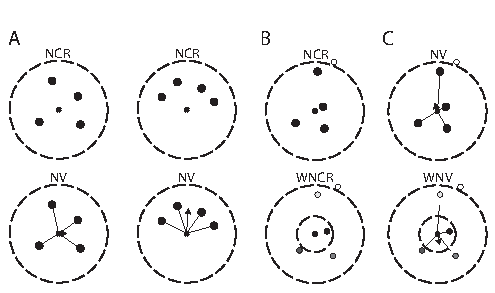
\includegraphics[width=4in]{figures/nv_kbp/nv_schematic}
\caption{
(A) The left and right panels both have the same ROSETTA neighbor count \citep{Dantas:2003vt} but very different degrees of burial.
The neighbor vector method is able to distinguish between these cases by calculating the vectors between the query residue and its neighbors.
The length of the vector indicates the degree of burial, with shorter vectors representing more buried residues. 
(B) The weighted NCR (WNCR) method gives a higher weight to neighbors near the query residue, smoothing the effect of small changes in composition on the measured degree of burial. 
(C) The combination of the NV and WNCR methods results in a more accurate measure of residue distribution. 
In all panels, dotted lines represent lower and upper bounds for counts, the X marks the query residue, and circles represent residues surrounding the query residue.
}
\label{fig:nv_schematic}
\end{figure}

The half sphere approximation method developed by Hamelryck in 2005 \citep{Hamelryck:2005kt} approximates surface accessibility by counting the number of residues in a half sphere below the side chain of each amino acid.
The half sphere count is directly related to residue burial.
Half Sphere Exposure (HSE) is implemented in the freely available BioPython library, and this library was used to compare performance of HSE and NV to relative SASA (calculated using NACCESS).
The per residue exposure was calculated for each of the proteins in the 42 protein benchmark set, and adjusted $R^{2}$ values were calculated for the correlation of each measure to relative SASA (rSASA).
The adjusted correlation factor $R^{2}$ value for HSE to rSASA was 0.68, while the adjusted correlation factor $R^{2}$ for the NV method was 0.86.
This suggests that while HSE is conceptually simpler, it does not perform as accurately as NV for proteins in our benchmark set.

A linear regression modeling the correlation between rSASA values (in the range of 0 to 1 calculated using NACCESS) and NV score (range 0 to 1) was generated based on all proteins in the 42 protein benchmark set.
The resulting linear regression model was rSASA = 1.29*(NV)-0.11 and had an $R^{2}$ of 0.86.
Based on this model, residues with NV scores between 0.00 to 0.24 will have an approximate rSASA value of 0 to 0.19, residues with NV scores from 0.25 to 0.39 will have an approximate rSASA value of 0.21 to 0.39, and residues with NV scores between 0.40 to 1.00 will have an approximate rSASA value of 0.40 to 1.10.

Terms in the RosettaDesign energy function can take the form of either single-body or two-body terms.
Two-body terms describe energies that pertain to the interaction between residues, such as the energy associated with hydrogen bonding, while single-body terms describe energies that pertain only to a single residue.
The resulting NV environment KBP was implemented as a single-body term in the RosettaDesign energy function.
RosettaDesign revision 39040 was used in all calculations.  

Computationally assessing the performance of a protein design algorithm is inherently challenging.
Historically, percent sequence recovery has been used as a metric for the quality of a protein design, as it has been observed that protein sequences are frequently close to optimal for a given fold\citep{Kuhlman:2000tc}.
However, many protein folds having large variations in sequence are frequently seen in nature \citep{Chothia:1986tm}.
Of the 74,608 protein chains present in the Structural Classification of Proteins (SCOP) database as of 2009, only 1,280 individual folds are observed \citep{Schaeffer:2011fe}.
In many positions, particularly on the surface of proteins, multiple residues can be tolerated with similar energies.
This finding limits sequence recovery as a measure for successful protein design because the design of a different but tolerated amino acid is counted as a failure.
To resolve this problem, we introduce a metric based on sequence homology. A Position Specific Scoring Matrix (PSSM) is derived from a Basic Local Alignment Search Tool (BLAST) query of the native sequence of a protein.
The percent recovery of amino acids with positive values in the PSSM determines recovery of evolutionarily tolerated amino acids. 

\section{Experimental Procedures}

The RosettaDesign energy function is a linear combination of individual energy terms.
As a result, the addition of a new energy term will impact the energy function as a whole.
To address this, each energy term is multiplied by a weight, and these weights must be carefully optimized following the introduction of a new term.
In most cases, it is not necessary to optimize the entire scoring function when a new term is added.
Instead, only the terms that describe similar information as the new term are optimized.
In the case of the NV environment KBP, the solvation free energy potential and the reference energies must also be optimized. 

To ensure that the optimized weights would apply to a wide range of proteins, a set of 100 soluble protein crystal structures from the Protein Data Bank (PDB) were used in optimization.
Structures were selected to have a sequence homology of less than 25\%, a length of 67-179 amino acids, and a resolution better than 2.0 \AA.
The optimization was conducted using a five-way cross validation protocol.
In this protocol, the 100 crystal structures described above were split into 5 groups of 20 structures each.
In each component of the five-way validation, 80 proteins were used during optimization, and the remaining 20 were used to benchmark the resulting weights.
In statistics generated from the benchmarking phase of the optimization process, results from all 5 sets of 20 proteins are combined, resulting in a total benchmark set of 100 proteins. 

An iterative particle swarm approach \citep{Chen:2007ua} was used to optimize the weights.
The RosettaDesign standard energy function was used as an initial point for optimization, and the weight of the NV environment KBP was arbitrarily given an initial weight of 1.0.
Twenty rounds of particle swarm optimization were performed for each component of the five-way cross validation described above.
The weights were optimized to maximize the PSSM score of proteins designed using the energy function (Table \ref{table:energy_weights}).
The PSSM for each protein was generated from a PSI-PRED BLAST query of the protein structure sequence using an e threshold of 0.001 and 3 iterations.
The non-redundant (NR) sequence database was used.
The average sequence identity between the query sequence and all other sequences in the generated PSSMs was 30\% for both benchmark sets.

\begin{table}
\scriptsize
\renewcommand{\tabcolsep}{0.09cm}
\centering
%This was supplement T1

\begin{tabular}{|r|r|r|r|r|r|r|r|r|r|}
\hline
& & & \multicolumn{5}{c|}{Five way cross validation sets} & &  \\
\hline
& Rosetta Scoring term & Scoring term description & 1 & 2 & 3 & 4 & 5 & Mean & Standard Deviation \\
\hline
\multirow{2}{*}{Free Weights} & fa\_sol & Solvation Free Energy Potential & 0.558 & 0.569 & 0.563 & 0.547 & 0.585 & 0.564 & 0.014 \\
\cline{2-10}
& neigh\_vect & NV environment KBP & 1.025 & 1.013 & 0.996 & 1.059 & 0.978 & 1.014 & 0.030 \\
\hline
\multirow{17}{*}{Fixed Weights} & fa\_atr & Attractive force & \multicolumn{5}{c|}{0.8} & 0.8 & 0.0\\
\cline{2-10}
& fa\_rep & Repulsive force & \multicolumn{5}{c|}{0.44} & 0.44 & 0.0\\
\cline{2-10}
& fa\_intra\_rep & Intra-residue repulsive force & \multicolumn{5}{c|}{0.004} & 0.004 & 0.0\\
\cline{2-10}
& pro\_close & Proline closure bonus & \multicolumn{5}{c|}{1.0} & 1.0 & 0.0\\
\cline{2-10}
& fa\_pair & Pair energy & \multicolumn{5}{c|}{0.49} & 0.49 & 0.0\\
\cline{2-10}
& hbond\_sr\_bb & Hydrogen bonding: short range backbone & \multicolumn{5}{c|}{0.585} & 0.585 & 0.0\\
\cline{2-10}
& hbond\_lr\_bb & Hydrogen bonding: long range backbone & \multicolumn{5}{c|}{1.17} & 1.17 & 0.0\\
\cline{2-10}
& hbond\_bb\_sc & Hydrogren bonding: backbone-sidechain & \multicolumn{5}{c|}{1.17} & 1.17 & 0.0\\
\cline{2-10}
& hbond\_sc & Hydrogen bonding: sidechain-sidechain & \multicolumn{5}{c|}{1.1} & 1.1 & 0.0 \\
\cline{2-10}
& dslf\_ss\_dst & Disulfide sidechain distance & \multicolumn{5}{c|}{1} & 1 & 0.0\\
\cline{2-10}
& dslf\_cs\_ang & Disulfide cystine sulfur angle & \multicolumn{5}{c|}{1} & 1 & 0.0\\
\cline{2-10}
& dslf\_ss\_dih & Disulfide sidechain-sidechain dihederal & \multicolumn{5}{c|}{1} & 1 & 0.0\\
\cline{2-10}
& dslf\_ca\_dih & Disulfide C?-sidechain dihederal & \multicolumn{5}{c|}{1} & 1 & 0.0\\
\cline{2-10}
& rama & Ramachandran score & \multicolumn{5}{c|}{0.2} & 0.2 & 0.0\\
\cline{2-10}
& omega & Omega angle score & \multicolumn{5}{c|}{0.5} & 0.5 & 0.0\\
\cline{2-10}
& p\_aa\_pp & Probability of an AA given phi/psi angle & \multicolumn{5}{c|}{0.32} & 0.32 & 0.0 \\
\cline{2-10}
& fa\_dun & dunbrack rotamer library & \multicolumn{5}{c|}{0.56} & 0.56 & 0.0\\
\hline
\end{tabular}
\caption{A table showing the individual weights included in the optimization, and their values in each of the five cross validation sets.  The mean and standard deviation of each free weight is also shown. }
\label{table:energy_weights}
\end{table}

Because the standard deviation of the averaged reference averaged reference energies was relatively high, the reference energies of the averaged energy function are optimized to reduce the overall sequence composition biases introduced during design (Tabel \ref{table:ref_energy_weights}).

Two separate optimization experiments were performed.
In the first experiment, the reference energies, solvation free energy potential, and the NV environment KBP were optimized.
In the second experiment, the NV environment KBP was excluded from the energy function, and only the reference energies were optimized.
This second experiment acts as a control and makes it possible to distinguish between design improvements due to reference energy optimization and design improvements due to the addition of the NV environment KBP itself.
While both NV environment KBP and the solvation free energy potential describe overlapping but different phenomena at different levels of resolution: The NV environment KBP is an indirect measure of solvation free energy and evolutionary biases against aggregation.
It is a measure at amino acid resolution and will be independent of side chain conformation.
In contrast, the solvation free energy potential is at atomic resolution incorporating a specific model of solvation.
While the solvation free energy potential does an inadequate job of accounting for biases against aggregation on the protein surface, it is highly accurate in avoiding burial of polar atoms, and is important to determine side chain conformation.

\begin{table}
\scriptsize
\renewcommand{\tabcolsep}{0.09cm}
\centering
%This was supplement T2
\begin{tabular}{|c|r|r|r|r|r|r|r|r|}
\hline
 \textbf{AA name} & \multicolumn{5}{c|}{\textbf{Five way cross validation sets}} & & &  \\
\hline
 & \textbf{1} & \textbf{2} & \textbf{3} & \textbf{4} & \textbf{5} & \textbf{Mean} & \textbf{Standard Deviation} & \textbf{Re-optimized Energies} \\
\hline
\hline
A & -0.313519 & -0.345577 & -0.332996 & -0.299376 & -0.311145 & -0.3205226 & 0.018489708 & -0.280778\\
\hline
C & -0.186065 & -0.267899 & -0.251004 & -0.203121 & -0.273443 & -0.2363064 & 0.039429392 & -0.191836\\
\hline
D & -0.0516543 & -0.152027 & -0.117976 & -0.04581 & -0.158867 & -0.10526686 & 0.053922242 & -0.0894836\\
\hline
E & -0.116794 & -0.225243 & -0.221177 & -0.13447 & -0.230275 & -0.1855918 & 0.055185343 & -0.163316\\
\hline
F & 0.979346 & 1.00881 & 1.09867 & 0.976394 & 1.03573 & 1.01979 & 0.05028824 & 1.0029\\
\hline
G & 0.187346 & 0.862973 & 0.681024 & 0.322192 & 0.952133 & 0.6011336 & 0.334354423 & 0.318222\\
\hline
H & 0.773425 & 0.727736 & 0.727848 & 0.755789 & 0.683065 & 0.7335726 & 0.034276949 & 0.738805\\
\hline
I & -0.0879415 & -0.063614 & -0.0662562 & -0.147069 & -0.0349584 & -0.07996782 & 0.041974551 & -0.0892347\\
\hline
K & -0.0356543 & -0.113405 & -0.125976 & -0.0465226 & -0.104256 & -0.08516278 & 0.041146221 & -0.0565743\\
\hline
L & -0.288888 & -0.27654 & -0.302976 & -0.350292 & -0.286631 & -0.3010654 & 0.029090569 & -0.295543\\
\hline
M & -0.475654 & -0.472027 & -0.532784 & -0.514173 & -0.478867 & -0.494701 & 0.027189556 & -0.488778\\
\hline
N & -0.523683 & -0.559673 & -0.549976 & -0.500635 & -0.582867 & -0.5433668 & 0.031950345 & -0.532584\\
\hline
P & -0.486622 & -0.556899 & -0.579705 & -0.488828 & -0.551983 & -0.5328074 & 0.042469908 & -0.494263\\
\hline
Q & -0.481516 & -0.58252 & -0.554953 & -0.491584 & -0.569756 & -0.5360658 & 0.046379036 & -0.497717\\
\hline
R & -0.280894 & -0.364054 & -0.324666 & -0.255467 & -0.389405 & -0.3228972 & 0.055748092 & -0.294276\\
\hline
S & -0.396296 & -0.436734 & -0.438423 & -0.37399 & -0.437601 & -0.4166088 & 0.029793151 & -0.393299\\
\hline
T & -0.312536 & -0.375408 & -0.373141 & -0.307255 & -0.368256 & -0.3473192 & 0.034311466 & -0.332279\\
\hline
V & -0.175465 & -0.166283 & -0.166976 & -0.217204 & -0.134509 & -0.1720874 & 0.029660029 & -0.176609\\
\hline
W & 1.43079 & 1.50528 & 1.52902 & 1.46971 & 1.42618 & 1.472196 & 0.045170863 & 1.47413\\
\hline
Y & 0.842276 & 0.853102 & 0.902422 & 0.851712 & 0.81571 & 0.8530444 & 0.031423486 & 0.842514\\
\hline

\end{tabular}

\caption{A table showing the optimized weights of the reference energies for each amino acid. }
\label{table:ref_energy_weights}
\end{table}


The optimization experiments described above produce 5 individual energy functions, each generated from one section of the five-way cross validation.
To produce a single optimized scoring function for general use, the weights from the 5 optimized energy functions are averaged together, and the reference energies of the averaged energy function are optimized using the set of 100 proteins used in the initial  cross validation.
The averaged energy function is benchmarked on an independent set of 42 protein crystal structures, in which the proteins have a sequence homology of less than 15\%, a size range of 150-225, and a resolution less than 1.5 \AA.
Note that these proteins are larger and more complex than the proteins used in the more time-consuming weight optimization procedure.
As a result, this benchmark poses a formidable challenge for the RosettaDesign fixed backbone design algorithm.
Several different metrics were used during benchmarking to assess the quality of designed proteins.
Percent PSSM recovery was the primary benchmarking metric used in the study.
Percent PSSM recovery was calculated as the percentage of residues that were designed as residues with a positive score in the PSSM of the native protein.
In addition, the percent sequence recovery was measured as the percentage of residues that remained in as the native residue after design. 

The percent PSSM recovery per residue, percent sequence recovery per residue, and the change in overall sequence composition were also calculated for each designed protein.
Percent PSSM recovery per residue is calculated as $\frac{num\ pssm\ recovered}{num\ designed}$ where $num\ pssm\ recovered$ is the number of residues with a given identity which were designed to a residue with a positive PSSM score, and $num\ designed$ is the total number of residues designed. 
Percent sequence recovery per residue was calculated as $\frac{num\ recovered}{num\ designed}$ where $num\ recovered$ is the number of residues with a given identity which were designed to an identical residue.
In addition to calculating overall percent sequence recovery, sequence recovery by chemical group was also calculated.
In this metric, residues were grouped into the categories polar (Ser, Thr, Asn, Gln), non-polar (Ala, Val, Leu, Met, Ile), aromatic (Phe, Tyr, Trp), charged (Lys, Arg, His, Asp, Glu), and other (Cys, Pro, Gly). 
A residue was counted as recovered if it was mutated to another residue within the same group.

Percent sequence composition change per amino acid type was calculated as $\frac{d-n}{num\ designed}$ where $d$ is the count of designed residues of a given type, and $n$ is the count of native residues.
To compute the change in overall sequence composition, a root mean square (RMS) deviation method was used.
RMS percent sequence composition change was calculated as follows, where $statistical\ metric$ is one of the metrics described above (shown as black bars in figures \ref{fig:overall_crossval_changes} and \ref{fig:overall_independent_changes}):

\begin{equation}
RMS=\sqrt{\frac{1}{20}\sum^{20}_{i=1..20}(statistical\ metric)^{2}}
\end{equation}

All of the above metrics were calculated for the entire protein, as well as the deeply buried region, surface region, and a boundary layer between the two.
For this study, the buried region is defined as all residues with a NV score between 0.00 and 0.24, the boundary is defined as 0.25 to 0.39, and the surface region is defined as 0.40 to 1.00.
The performance of the optimized energy functions via these benchmarks was compared to the performance of the standard RosettaDesign energy function.

The benchmarks described above are intended as a measure of how well RosettaDesign is accomplishing its goal of generating low-energy, native-like protein sequences.
In a well-optimized energy function, we expect that the percent PSSM recovery will increase compared to the standard RosettaDesign energy function.
We also expect that the percent sequence recovery will remain similar to that obtained with the standard energy function.
Finally, we expect that a well-optimized energy function will exhibit smaller biases in sequence composition compared to proteins designed with the standard energy function.

\section{results}

The percent PSSM recovery and percent sequence recovery calculated for the 100 proteins used in the five-way cross validation are shown in Table \ref{table:burial_100}.
The results of PSSM recovery and sequence recovery analysis show that the optimized NV environment KBP energy function exhibits a 5.2\% improvement in percent PSSM recovery compared to the standard energy function and that 3.6\% of this improvement was a result of reference energy optimization.
The NV environment KBP energy function showed a 1.6\% improvement in percent sequence recovery compared to the standard RosettaDesigne energy function and a 2.4\% improvement if only reference energies are optimized.  

\begin{table}
\scriptsize
\renewcommand{\tabcolsep}{0.09cm}
\centering
\begin{tabular}{|r||r|r|r|r|r|r|}
\hline
 & \multicolumn{3}{c}{\textbf{Percent PSSM Recovery}} & \multicolumn{3}{|c|}{\textbf{Percent Sequence Recovery}}\\
\hline
  & \textbf{Standard} & \textbf{Reference} & \textbf{NV environment KBP} & \textbf{Standard} & \textbf{Reference} & \textbf{NV environment KBP}\\
\hline
\hline
Buried & 73.4\% & 77.1\% & 78.9\% & 64.9\% & 66.5\% & 65.5\% \\
\hline
Boundary & 72.1\% & 75.3\% & 77.3\% & 44.3\% & 46.6\% & 45.5\% \\
\hline
Surface & 70.4\% & 74.4\% & 75.9\% & 32.8\% & 35.9\% & 35.5\% \\
\hline
Overall & 72.0\% & 75.6\% & 77.2\% & 45.7\% & 48.1\% & 47.3\% \\
\hline
\end{tabular}
\caption{Percent PSSM recovery and percent sequence recovery by degree of burial for 100 proteins used in optimization. "Standard" refers to the standard energy function, "Reference" refers to the modified standard energy function in which the reference energies were re-optimized, and "NV environment KBP" refers to the optimized energy function incorporating the NV environment energy term.}
\label{table:burial_100}
\end{table}

The percent change in composition between native and designed sequences for the 100 proteins used in the five-fold cross-validation is shown in Figure \ref{fig:overall_crossval_changes}A.
Proteins designed with the NV environment KBP energy function show a decrease in the average magnitude of sequence composition biases introduced during design compared to proteins designed with the standard energy function.
Proteins designed with the standard energy function exhibit an RMS percent change in sequence composition of 2.0\%, while proteins designed with the NV environment KBP show an RMS percent change in sequence composition of 1.0\%.
Figure \ref{fig:overall_crossval_changes}B shows that RMS per residue PSSM recovery increased from 3.8\% with the standard energy function to 4.2\% with the NV environment KBP, and \ref{fig:overall_crossval_changes}C shows that RMS per residue sequence recovery remained relatively constant between the standard energy function and NV environment KBP. 

\begin{figure}
\centering
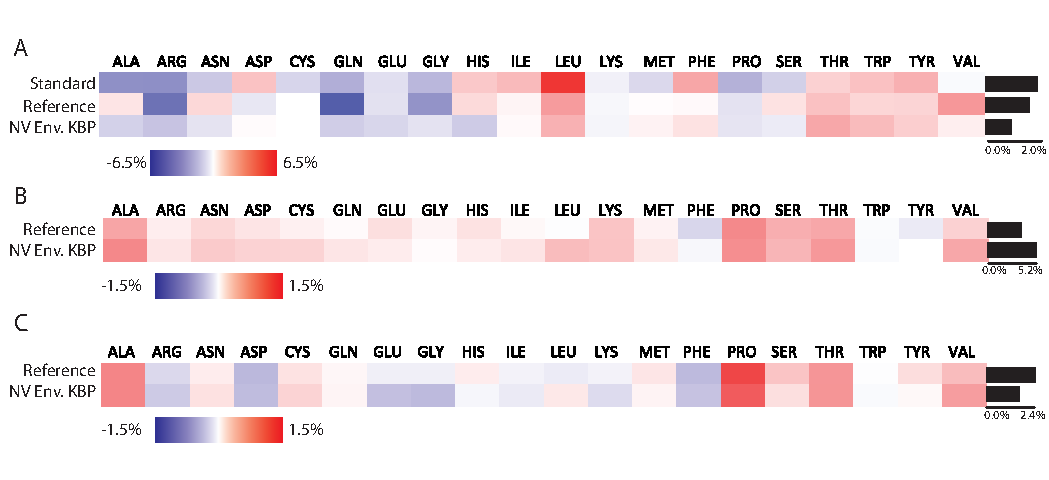
\includegraphics[width=4in]{figures/nv_kbp/overall_crossval_changes}
\caption{
A) shows the percent change in overall sequence composition between native and designed proteins for all 100 structures in the five-way cross-validation set.
The black bars show the RMS percent composition change.
B) shows the percent PSSM recovery for all 100 structures in the five-way cross-validation set.  The black bars show RMS percent PSSM recovery.
C) percent sequence recovery for all 100 structures in the five-way cross-validation set.  The black bars show RMS percent sequence recovery.	
}
\label{fig:overall_crossval_changes}
\end{figure}


The energy functions produced with the five-way validation were averaged to produce a single energy function, the reference energies of this averaged function were optimized, and the benchmarking analysis used above was repeated using the averaged energy function.
In this case, the independent benchmark set of 42 proteins was used.
Table \ref{table:burial_42} shows the percent PSSM recovery and percent sequence recovery calculated for the 42 proteins designed using the averaged energy function.
The NV environment KBP showed an 8.8\% improvement in PSSM recovery compared to the standard energy function and that 3.8\% of this improvement was a result of the reference energy optimization.
The NV environment KBP showed a 3.2\% overall improvement in sequence recovery of which 1.9\% was due to the reference energy optimization. 

\begin{table}
\scriptsize
\renewcommand{\tabcolsep}{0.09cm}
\centering
\begin{tabular}{|r|r|r|r|r|r|r|}
\hline
 & \multicolumn{3}{c}{Percent PSSM Recovery} & \multicolumn{3}{|c|}{Percent Sequence Recovery}\\
\hline
  & Standard & Reference & NV environment KBP & Standard & Reference & NV environment KBP \\
\hline
Buried & 68.0\% & 70.7\% & 76.0\% & 49.5\% & 49.8\% & 51.5\% \\
\hline
Boundary & 66.1\% & 70.6\% & 75.7\% & 32.1\% & 34.1\% & 35.3\% \\
\hline
Surface & 67.2\% & 72.2\% & 75.8\% & 22.7\% & 26.3\% & 27.3\% \\
\hline
Overall & 67.4\% & 71.2\% & 75.9\% & 35.7\% & 37.6\% & 38.9\% \\
\hline
\end{tabular}
\caption{Percent PSSM recovery and percent sequence recovery by degree of burial for 42 proteins used in benchmarking. 
"Standard" refers to the standard energy function, "Reference" refers to the modified standard energy function in which the reference energies were reoptimized, and "NV environment KBP" refers to the optimized energy function incorporating the NV environment energy term.}
\label{table:burial_42}
\end{table}

When sequence recovery is broken down by group (Figure \ref{fig:recovery_by_group} ), a large improvement (decrease) in the percentage of unrecovered buried charged residues is observed, from 8.78\% to 1.96\% unrecovered residues function in the 100 protein benchmark set.
Additionally, a decrease from 8.77\% to 3.46\% unrecovered non-polar residues on the surface is observed.
Additionally, Figure \ref{fig:recovery_by_group} reveals a fundamental difference in the two datasets.
The lower recovery values seen in all categories in the 42-protein benchmark set suggest that it is a much more challenging target for design than the 100-protein benchmark set used in optimization.
The proteins of the 42-protein benchmark set are substantially larger (average length of 207 residues) than those in the 100-protein benchmark set (average length of 120 residues).
Each additional residue drastically increases the number of possible sequences to consider, decreasing the probability of a high quality design.
Despite this more challenging independent benchmark, improvement was still observed. 

\begin{figure}
\centering
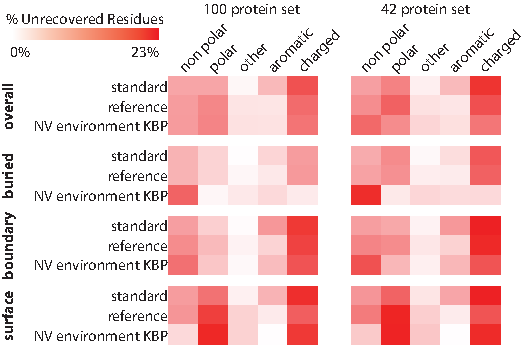
\includegraphics[width=4in]{figures/nv_kbp/recovery_by_group}
\caption{
Percentage of unrecovered residues (number of recovered residues divided by total number of residues in the benchmark set) by amino acid category in the 100 and 42 protein benchmark sets.
The color scale ranges from white (small number of mistakes) to red (large number of mistakes).
In this metric, residues were grouped into the categories polar (Ser, Thr, Asn, Gln), non-polar (Ala, Val, Leu, Met, Ile), aromatic (Phe, Tyr, Trp), charged (Lys, Arg, His, Asp, Glu), and other (Cys, Pro, Gly).
A residue was counted as recovered if it was mutated to another residue within the same group.
}
\label{fig:recovery_by_group}
\end{figure}

\section{Discussion}

The results of both the 100-protein five-way cross-validation and the 42-protein independent benchmark set are consistent.
In both cases, introduction of the NV environment KBP into the energy function and optimization of the energy function weights lead to an overall improvement in the quality of designed sequences.
As the independent benchmark set tests an averaged scoring function that would be generally useful, the remaining analysis will focus on this benchmark set. 

The results of the benchmarking show that, in general, structures designed using the NV environment KBP exhibit smaller conformation biases and more evolutionarily favorable mutations.
A detailed analysis of these results also provides some insight into the behavior of the RosettaDesign scoring function.

Due to the lack of an explicit water model in RosettaDesign, the standard RosettaDesign energy function is dominated by the solvation free energy potential.
As a result, there are few constraints on amino acid mutations on the protein surface.
Due to this lack of constraints, proteins designed with the standard energy function exhibit large biases in sequence composition on the protein surface.
Proteins designed with the standard energy function show large numbers of aromatic residues on the protein surface.
Specifically, there is a 3.1\% increase in phenylalanines, a 1.9\% increase in tryptophans, and a 2.5\% increase in tyrosines on the protein surface in the benchmark set designed with the standard RosettaDesign energy function compared to the native structure.
Proteins designed with the NV environment KBP show a large reduction in these biases.
Proteins designed with the NV environment KBP showed a 1.4\% increase in phenylalanines, 0.8\% increase in tryptophans, and 1.5\% increase in tyrosines compared to native proteins.
While still large, these biases are much smaller than the biases observed with the standard energy function. 

It was expected that improvements in the quality of surface sequence design would be the primary benefit of the NV environment KBP.
However, an analysis of the overall PSSM recovery, sequence recovery, and sequence composition biases suggest that the improvement given by the NV environment KBP implementation occurred across the board rather than merely at the protein surface.
Table \ref{table:burial_42} shows the overall impact of the NV environment KBP at various levels of burial.
The percent PSSM recovery improved using the NV environment KBP by 8.0\% in the buried region, 9.6\% in the boundary region, and 8.5\% on the surface region compared to the standard energy function.
The percent sequence recovery improved by 2.0\% in the buried region, 3.2\% in the boundary region, and 4.6\% in the surface region compared to the standard energy function.
 
 When percent sequence recovery is broken down by group (Figure \ref{fig:recovery_by_group}), a large increase in the recovery of buried charged residues is observed, with a 6.2\% increase compared to the standard energy function. 
 Additionally, a 3.8\% increase in recovery of non-polar residues is observed on the surface.
 Not all groups show improvement, and this is expected, as the scoring function was not directly optimized for percent sequence recovery.
 
While the overall percent changes are relatively small, these changes are both statistically and scientifically significant.
To assess the statistical significance of the data, standard deviations were calculated in tables \ref{table:100_protein_stdev} and \ref{table:42_protein_stdev}.
The standard deviations were calculated for both percent PSSM recovery and percent sequence recovery.
Each of the five scoring functions generated during the five-way cross validation weight optimization using 100 proteins was used to design the independent set of 42 proteins.
The standard deviations of PSSM and sequence recovery are listed in supplementary tables \ref{table:100_protein_stdev} and \ref{table:42_protein_stdev}.
The standard deviations range from 0.1-1.2\%. 
The average error is 0.4\% and therefore smaller that the improvements in recovery rates observed. 

\begin{table}
\scriptsize
\renewcommand{\tabcolsep}{0.09cm}
\centering
%This was table T3

\begin{tabular}{|r|r|r|r|r|r|r|}
\hline
 & \multicolumn{3}{c}{Percent PSSM Recovery} & \multicolumn{3}{|c|}{Percent Sequence Recovery}\\
\hline
  & Standard & Reference & NV environment KBP & Standard & Reference & NV environment KBP \\
\hline
Buried & 8.9\% & 8.9\% & 8.4\% & 11.6\% & 10.8\% & 10.1\%\\
\hline
Boundary & 9.6\% & 11.7\% & 9.2\% & 10.7\% & 11.3\% & 11.2\%\\
\hline
Surface & 8.1\% & 6.6\% & 6.9\% & 7.0\% & 8.0\% & 7.9\%\\
\hline
Overall & 6.3\% & 6.0\% & 5.2\% & 7.0\% & 7.1\% & 6.5\%\\
\hline
\end{tabular}
\caption{Standard deviations for 100 protein benchmark set data. shown in table \ref{table:burial_100}}
\label{table:100_protein_stdev}
\end{table}

\begin{table}
\scriptsize
\renewcommand{\tabcolsep}{0.09cm}
\centering
%This was table T4

\begin{tabular}{|l||r|r|r|r|r|r|}
\hline
 & \multicolumn{3}{c}{\textbf{Percent PSSM Recovery}} & \multicolumn{3}{|c|}{\textbf{Percent Sequence Recovery}}\\
\hline
  & \textbf{Standard} & \textbf{Reference} & \textbf{NV environment KBP} & \textbf{Standard} & \textbf{Reference} & \textbf{NV environment KBP} \\
\hline
\hline
Buried & 7.1\% & 6.7\% & 5.9\% & 8.1\% & 8.9\% & 7.7\%\\
\hline
Boundary & 9.2\% & 9.1\% & 8.7\% & 8.1\% & 8.0\% & 8.6\%\\
\hline
Surface & 6.9\% & 6.6\% & 7.4\% & 4.7\% & 6.8\% & 6.0\%\\
\hline
Overall & 5.5\% & 5.7\% & 5.7\% & 4.6\% & 5.5\% & 5.3\%\\
\hline
\end{tabular}
\caption{Standard deviations for 42 protein benchmark set data. shown in table \ref{table:burial_42}}
\label{table:42_protein_stdev}
\end{table}

It is important to consider not only the absolute change in percent recovery, but also the change relative to the maximum possible recovery value.
In the case of sequence recovery, the maximum possible sequence recovery can be estimated by analyzing the amino acids tolerated in each position in BLAST derived PSSMs.
In this case, the average percentage of time that the native residue is seen in the PSSM is used as an estimate for expected sequence recovery.
For the 100 protein benchmark set, the average was 34\%, with a standard deviation of 12\%, while in the 42 protein benchmark set, the average was 34\% with a standard deviation of 7\%.
While the achievable sequence recovery is somewhat higher due to correlation between individual positions, these values suggest that obtaining sequence recovery rates of 40-50\% would approach the maximum.
Tables \ref{table:burial_100} and \ref{table:burial_42} show that for the 100 protein benchmark set, total overall sequence recovery is 45.7\% with the standard energy function and 47.0\% with the NV environment KBP.
For the 42 protein benchmark set, total overall sequence recovery is 35.7\% with the standard energy function and 38.9\% with the NV environment KBP.
This explains the relatively small increases in sequence recovery, as current recovery values are approaching the practical maximum.
For that reason we introduce the PSSM recovery value.
In this context it is important to note that the scoring functions were not directly optimized for sequence recovery but rather PSSM recovery.
As a result, it is not surprising that the sequence recovery is not necessarily maximized during optimization. 

In the case of PSSM recovery, it is reasonable to expect that 100\% PSSM recovery is unreachable as evolution might not have sampled all amino acids tolerated in a sequence position.
A more realistic value for maximum possible PSSM recovery is between 80\% and 90\%, though the exact value of this upper bound is difficult to estimate. PSSM recovery with the standard energy function was 72.0\%.
The observed increase to 77.2\% with the NV environment KBP represents a substantial increase relative to the 80-90\% maximum and the 72\% starting point.
Generally, improvements in sequence recovery rates have been moderate when altering the energy function \citep{Kortemme:2003td}, as the major contributors to the overall energy are already fine-tuned and remain unaltered. 

Comparison of PSSM and sequence recovery results between the 42 protein benchmark set and the 100 protein set illustrates that the performance of the RosettaDesign algorithm varies based on the characteristics of the protein being designed.
For example, Table \ref{table:burial_100} and \ref{table:burial_42} show the overall sequence recovery for proteins designed with the standard energy function.
The overall recovery for the 42 protein benchmark set was 35.7\%, while the overall recovery for the 100 protein benchmark set was 45.7\%.
This substantial difference is likely a result of the different criteria used to select the proteins in each set.
The proteins in the 42 protein benchmark set are larger than those in the 100 protein set, and will therefore have a larger total surface area and thus be more challenging targets for design.

Despite the difference inherent to different design targets, these values are similar to those obtained in the literature.
Schneider et al. designed a set of proteins of size between 89-223 amino acids based on high resolution crystal structures.
They observed surface sequence recovery rates of 22\%+/- 11\%, and buried recovery rates of 56\%+/- 13.7\% when designing with RosettaDesign \citep{Schneider:2009ig}.
These values are similar to those seen in Tables \ref{table:burial_100} and \ref{table:burial_42}.
Additionally, Sharabi et al. reported overall sequence recovery values of between 40\% and 70\% depending on the weights of the scoring function used during their design \citep{Sharabi:2011ev}.
These numbers are within the range of the sequence recovery values obtained during the experiments described in this manuscript.

In addition to improvements in PSSM and sequence recovery, the degree of sequence bias seen in the buried and boundary regions of designs made using the NV environment KBP decreased.
When all residues in the benchmark set are considered, proteins designed with the NV environment KBP have an RMS percent composition change of 2.8\% compared to the native protein, while proteins designed with the standard energy function have an RMS percent composition change of 2.9\% (Figure \ref{fig:overall_independent_changes}A).
When this overall value is broken down by region, the buried region designed with the NV environment KBP shows an increase in RMS percent composition change compared to the standard energy function from 4.2\% to 4.5\%, the boundary region shows a decrease from 3.4\% to 2.7\%, and the surface region shows a reduction from 2.9\% to 2.4\%.
While the improvements in sequence composition bias are minimal, Figure \ref{fig:overall_independent_changes}B shows an increase in RMS per residue PSSM recovery from 3.8\% with the standard energy function to 4.2\% with the NV environment KBP.
Additionally, Figure \ref{fig:overall_independent_changes}C shows an increase in RMS per residue sequence recovery from 2.4\% with the standard energy function to 2.6\% with the NV environment KBP energy function, which is expected given the optimization of the scoring function towards PSSM improvement. 

\begin{figure}
\centering
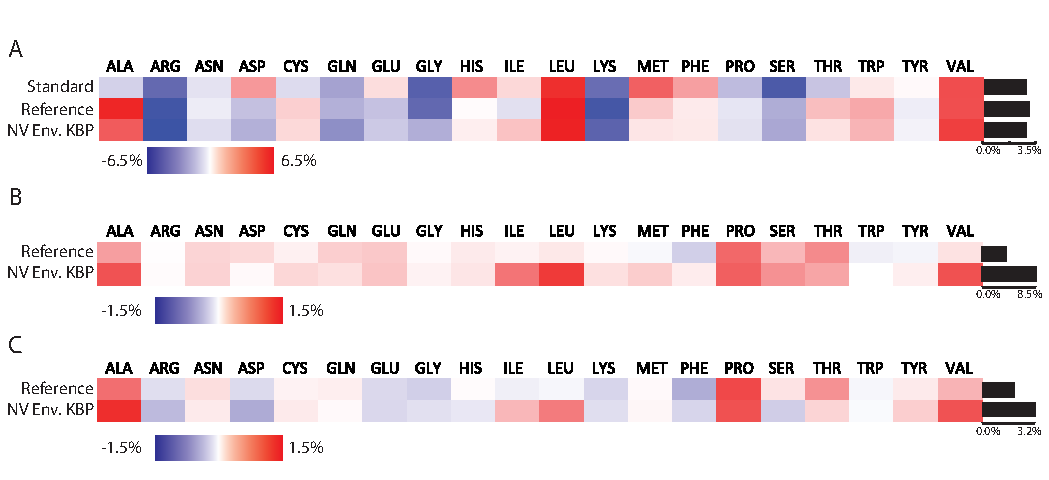
\includegraphics[width=4in]{figures/nv_kbp/overall_independent_changes}
\caption{
A) shows the percent change in overall sequence composition between native and designed proteins for all 42 structures in the independent benchmark set.
The black bars show the RMS percent composition change. 
B) shows the percent PSSM recovery for all 42 structures in the independent benchmark set.
The black bars show RMS percent PSSM recovery.  
C) percent sequence recovery for all 42 structures in the independent benchmark set.
The black bars show RMS percent sequence recovery.
}
\label{fig:overall_independent_changes}
\end{figure}
 
An investigation of the optimized weights lends some insight into the cause of the improvements in sequence design.
 Table \ref{table:energy_weights} and \ref{table:ref_energy_weights} show the scoring function and reference energy weights of the standard energy function and the optimized NV environment KBP.
When the NV environment KBP term is added to the energy function, the weight of the free energy solvation potential decreases from 0.65 in the standard energy function to 0.56 in the NV environment KBP. 
The NV environment KBP term has a value of 1.01.
As discussed earlier, in the standard energy function, the reference energies and solvation free energy potential are the dominant forces on surface residues due to the lack of explicit inter-residue interactions.
Because the penalty given by the solvation free energy potential for apolar residues on the surface is relatively weak, the weight of this potential will need to be increased for it to adequately effect surface residues.
However, because the energy function is applied evenly, regardless of degree of burial, the increase in weight necessary to maintain a reasonable protein surface may cause the solvation free energy potential to apply too strongly to the boundary region.
As the burial level increases, the number of inter-residue interactions will also increase, which explains the decrease in improvement in sequence bias seen at more highly buried regions of the protein.
This idea is supported by the decrease in free energy solvation potential weight observed in the NV environment KBP energy function.
The NV environment KBP provides additional information about protein surface composition, reducing the dominance of the free energy solvation potential.

\begin{figure}
\centering
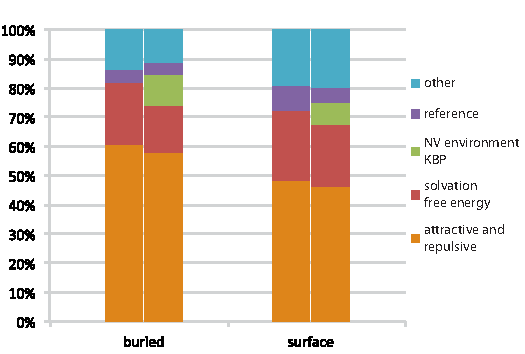
\includegraphics[width=4in]{figures/nv_kbp/term_contribution}
\caption{
The contribution of individual scoring terms towards the overall score of buried and surface residues.
The introduction of the NV environment KBP reduces the reliance on solvation free energy and the attractive/repulsive forces at both levels of exposure. 
}
\label{fig:term_contribution}
\end{figure}

Figure \ref{fig:term_contribution} shows the effect of the NV environment KBP on the overall scoring function.
All proteins used in the 100 protein benchmark set were scored using both the standard RosettaDesign energy function and the optimized NV environment KBP energy function. 
The average magnitude of each scoring term for each buried and surface residue was calculated, and converted to percentage of the total energy for each residue to measure the influence of each scoring term.
We observe that the addition of the NV environment KBP term decreases the influence of the reference energies, solvation free energy term, and the attractive and repulsive terms throughout all degrees of burial.
Specifically, the influence of the solvation free energy decreases from 21\% to 16\% for buried residues, and from 24\% to 21\% for surface residues.
Additionally, the influence of the reference energy decreases from 8\% to 5\% on the surface, though it remains relatively unchanged for buried residues.
The attractive and repulsive forces also change somewhat, with a decrease in influence from 60\% to 57\% in buried residues, and 48 to 46\% in surface residues.
This change in influence is significantly less than the change in influence seen in the reference and solvation free energy functions.
The NV environment KBP was designed to address shortcomings in the design of the protein surface.
These shortcomings are the result of the energy function failing to model aspects of the protein surface that are not completely described through the solvation and reference energies.
To achieve reasonably good performance despite these inaccuracies, both energy terms are overweighted in the standard energy function.
As expected, addition of the NV environment KBP term reduces the impact of solvation and reference energies on the surface.
As these adjustments apply throughout all degrees of burial, the artificially inflated weight of the solvation and reference energies can be decreased, improving performance also in the buried regions of the protein as well.

In addition to providing information about solvation effects, the NV environment potential also sheds light on the evolutionary and environmental forces on protein composition.
Soluble proteins have evolved to be non-aggregative and generally stable in the environment of a cell.
These properties are difficult to model via physics-based methods, as they arise from numerous inter-protein interactions that are difficult to explicitly model.
The implicit modeling of these environmental effects accounts in part for the improvements in native-like sequence design seen during design with the NV environment KBP.
By optimizing the NV environment KBP energy function to maximize PSSM score rather than sequence recovery, the energy function is optimized to design proteins similar to those which are favored evolutionarily, rather than to merely reproduce the native sequence.